\chapter{Sistemi di trasmissione numerica}
Un \keyword[sistema di trasmissione!numerico]{sistema di trasmissione numerico} può essere utilizzato per trasmettere qualunque tipo di informazione codificata in una stringa di simboli numerici binari $1$ e $0$. Tali simboli generati da una sorgente con una certa velocità o \keyword[bit rate]{bitrate} in $\si{\bit\per\second}$, vengono trasformati a livello fisico in forme d'onda analogiche, e, affette da disturbi e rumore del canale di trasmissione, giungono al ricevitore. 

Al ricevitore non interessa ricostruire fedelmente le forme d'onda trasmesse ma è necessario elaborare e campionare il segnale per decidere in ogni intervallo di tempo quale simbolo si è ricevuto e poter ricostruire, con una certa probabilità di errore, la sequenza numerica dei simboli trasmessi.

\begin{figure}[!ht]
	\centering
	\resizebox{\textwidth}{!}{
		\begin{tikzpicture}[>=latex']
		\coordinate(c0);
		\node[block,right=1.5cm of c0](b0){GFO};
		\node[block,right=1.5cm of b0](b1){MT};
		\node[sum,right=1cm of b1](s0){$+$};
		\coordinate[above=1cm of s0](n);
		\node[block,right=1.5cm of s0](b2){FR};
		\node[campionatore,right=1cm of b2](q0){};
		\node[block,right=1cm of q0](b3){DEC};
		\coordinate[right=1.5cm of b3](c1);
		\draw[->](c0)--node[above,near start]{bit}(b0);
		\draw[dot=O](b0)--(b1);
		\draw[->](b1)--(s0);
		\draw[->](n)node[above]{$n(t)$}--(s0);
		\draw[dot=A](s0)--(b2);
		\draw[dot=B](b2)--(q0);
		\draw[dot=C](q0)--(b3);
		\draw[->](b3)--node[above,near end]{bit}(c1);
		\node[fitted, fit=(b0),label=above:Trasmettitore]{};
		\node[fitted, fit=(b1)(s0),label=above:Canale]{};
		\node[fitted, fit=(b2)(q0)(b3),label=above:Ricevitore]{};
		\end{tikzpicture}
	}
	\caption{Schema sistema di trasmissione numerico in banda base}
	\label{fig:schema_sistema_trasmissione_numerico_banda_base}
\end{figure}

Se il generatore di forme d'onda genera una tensione maggiore di zero per $T$ secondi per codificare “1” e una tensione nulla per $T$ secondi per codificare “0” si è in una condizione analoga a quella del sistema \ac{RADAR}: l'assenza di bersaglio corrisponde in ricezione al solo rumore tradotto nel simbolo “0”, la presenza di bersaglio corrisponde alla ricezione di segnale rumoroso sovrapposto alla forma d'onda ritardata e attenuata da interpretare come simbolo “1”.

In generale si può supporre di trasmettere una forma d'onda $s_0(t)$ per codificare il simbolo “$0$” e una forma d'onda diversa $s_1(t)$ per l'“$1$”. In tal caso al ricevitore si avranno due filtri che applicati ai due segnali forniranno due diverse uscite che vengono confrontate per decidere quale segnale è stato trasmesso.

Un filtro del ricevitore può essere adattato massimizzando l'uscita di tensione in corrispondenza del segnale che codifica per il simbolo da riconoscere. Per ricostruire la sequenza di bit in uscita si campiona l'uscita del filtro ad intervalli regolari con lo stesso ritmo della sorgente, e si determina il simbolo statisticamente più probabile con il decisore a soglia. La soglia è posta in modo tale da rendere equiprobabile l'errore di decisione.

\begin{figure}[ht!]\centering
\foreach\avg/\var in{1/0.707,1/0.5,2/.707} {
\subfloat[$\rho=\avg, \sigma^2=\var$]{
\begin{tikzpicture}
\begin{axis}[scale=.66,clip=false,xlabel=$V$,hide y axis,axis x line=middle,xtick={-\avg,\avg},ytick=\empty,xticklabels={$v_0$,$v_1$},extra x ticks={0.},extra x tick labels={soglia},extra x tick style={grid=major},samples=300,domain=-\avg-.5:\avg+.5]
\addplot [name path=gauss0] {gauss(x,-\avg,\var)};
\addplot [name path=gauss1] {gauss(x,\avg,\var)};
\path[name path=axis] (axis cs:-2.5,0)--node[above right,pos=0.5,pin=60:\footnotesize $P(1_R|0_T)$]{}node[above left,pos=0.5,pin=120:\footnotesize $P(0_R|1_T)$]{}(axis cs:2.5,0);
\addplot[pattern=north west lines] fill between[of=gauss0 and axis,soft clip={domain=0:2}];
\addplot[pattern=north east lines] fill between[of=gauss1 and axis,soft clip={domain=-2:0}];
\end{axis}
\end{tikzpicture}
}}
\caption{Modello statistico della decisione}
\label{fig:trasmissione_numerica_modello_statistico_decisione}
\end{figure}

Nei sistemi a trasmissione numerica la probabilità di commettere un errore su un simbolo è funzione del \ac{SNR} in ricezione:
\begin{equation}
p(\epsilon) = p(0_T)p(1_R|0_T)+p(1_T)p(0_R|1_T)
\end{equation}

Per ipotesi l'informazione contenuta nel segnale trasmesso avrà simboli 0 e 1 equiprobabili. Le probabilità condizionate corrispondono alle aree sottese alle code delle gaussiane suddivise dal valore di soglia.

Per ridurre la probabilità di errore si aumenta la distanza tra i picchi nella densità di probabilità in uscita ai filtri o si riduce la varianza dell'errore, utilizzando filtri a banda stretta.

Un filtro in ricezione a banda stretta limita l'energia passante del rumore ma anche la massima velocità di variazione del segnale, quindi un periodo minimo di tempo per ogni simbolo, ovvero il \keyword{bitrate}.

\section{Codifica ortogonale e antipodale}
Si possono scegliere le due forme d'onda $s_0(t)$ e $s_1(t)$ e i filtri adattati in modo tale che quando l'uscita di un filtro è massima l'altra sia nulla (\keyword{codifica ortogonale}). Ad esempio si può usare una forma d'onda per un simbolo e il valore costante nullo per l'altro.

In alternativa si può ottimizzare la potenza trasmessa facendo in modo che quando un'uscita è massima e positiva l'altra sia massima e negativa (\keyword{codifica antipodale}): ad esempio si può usare la stessa forma d'onda cambiata di segno per i due simboli. A parità di potenza di picco sarà immediato per il decisore determinare e confrontare, con la minore probabilità d'errore, il segno della tensione d'uscita ai filtri.

\begin{figure}[h!]
	\centering
	\begin{tikzpicture}[>=latex',thick];
	\coordinate(c0);
	\coordinate[below=1cm of c0](c2);
	\coordinate[below=1cm of c2](c1);
	\node [left=1cm of c2](n0){$s_R$};
	\draw (n0)--(c2)|-(c0)(c2)|-(c1);
	\node [block,right=1cm of c0](h0){$H_0(f)$} edge[<-](c0);
	\node [block,right=1cm of c1](h1){$H_1(f)$} edge[<-](c1);
	\coordinate[right=2cm of h0](c3);
	\coordinate[right=2cm of h1](c4);
	\node [block,minimum height=3cm,fit=(c3)(c4)](dec){$\lessgtr$};
	\coordinate[right=1cm of dec](u);
	\draw [->](h0)--(dec.126);
	\draw [->](h1)--(dec.235);
	\draw [->](dec)--node[above]{0}node[below]{1}(u);
	\end{tikzpicture}
	\caption{Schema di filtri adattati e decisore in ricezione per sistema di trasmissione numerica}
	\label{fig:trasmissione_numerica_filtri_adattati}
\end{figure}


\section{Pulse Amplitude Modulation}
Le forme d'onda che rappresentano i simboli binari di una trasmissione numerica possono essere segnali impulsivi modulati in ampiezza, o \ac{PAM}, scelti con codifica ortogonale o antipodale 
\[\begin{cases}0 \to n(t) \\ 1 \to s_1(t)+n(t)\end{cases} \quad \begin{cases}0 \to s_0(t)+n(t) \\ 1 \to s_1(t)+n(t)\end{cases} \]

Gli impulsi rettangolari sono la forma d'onda di base più semplice, con ampiezza costante di valore $s_0(t)=v_0$ o nullo per codificare uno “0” e valore $s_1(t)=v_1$ per codificare “1”.

Il segnale ricevuto affetto da rumore viene campionato ad intervalli regolari. Il ricevitore opera il campionamento utilizzando un segnale di sincronismo che indichi gli istanti in cui il segnale all'uscita del filtro adattato ha valore massimo. 

\`{E} possibile utilizzare un circuito integratore con azzeramento al campionatore per determinare il valore del campione alla fine di ogni periodo (tratteggiato in fig.\ref{fig:modulazione_numerica_PAM_ortogonale}c e \ref{fig:modulazione_numerica_PAM_antipodale}c).

\begin{figure}[ht!]\centering
\def\delay{.5}
\subfloat[Segnale trasmesso]{
	\begin{tikzpicture}[scale=.66]
	\begin{axis}[yscale=.5,xtick={},ytick={1},domain=0:7,ylabel=$s_T(t)$]
	\addplot[samples=125] {rect(x,1,2)+rect(x,3,5)};
	\end{axis}\end{tikzpicture}}\quad\subfloat[Segnale ricevuto]{
	\begin{tikzpicture}[scale=.66]
	\begin{axis}[yscale=.5,xtick={},ytick={1},domain=0:7,ylabel=$s_R^\text{A}(t)$]
	\addplot[samples=250] {noise(0,.1)+rect(x-\delay,1,2)+rect(x-\delay,3,5)};
	\end{axis}\end{tikzpicture}}%
\quad\subfloat[Segnale campionato]{
	\begin{tikzpicture}[scale=.66]
	\begin{axis}[yscale=.5,xtick={},ytick={1},domain=0:7,ylabel=$s_R^\text{C}(t)$]
	\addplot[samples=250] {noise(0,.1)+ramp(x-\delay,1,2)-ramp(x-\delay,2,3)+ramp(x-\delay,3,4)-ramp(x-\delay,5,6)};
	\addplot[only marks,mark=x,red] coordinates {(\delay,0)(\delay+1,0)(\delay+2,1)(\delay+3,0)(\delay+4,1)(\delay+5,1)(\delay+6,0)};
	\addplot[samples=125,dashed] {ramp(x-\delay,1,2)-grad(x-\delay,2)+ramp(x-\delay,3,4)-grad(x-\delay,4)+ramp(x-\delay,4,5)-grad(x-\delay,5)};
	\end{axis}\end{tikzpicture}}
\caption{Esempio di \acl{PAM} con codifica ortogonale}
\label{fig:modulazione_numerica_PAM_ortogonale}
\end{figure}

\begin{figure}[ht!]\centering
	\def\delay{.5}
	\subfloat[Segnale trasmesso]{
		\begin{tikzpicture}[scale=.66]
		\begin{axis}[yscale=.5,xtick={},ytick={1},domain=0:7,ylabel=$s_T(t)$]
		\addplot[samples=125] {-rect(x,0,1)+rect(x,1,2)-rect(x,2,3)+rect(x,3,5)};
		\end{axis}\end{tikzpicture}}\quad\subfloat[Segnale ricevuto]{
		\begin{tikzpicture}[scale=.66]
		\begin{axis}[yscale=.5,xtick={},ytick={1},domain=0:7,ylabel=$s_R^\text{A}(t)$]
		\addplot[samples=250] {noise(0,.1)-rect(x-\delay,0,1)+rect(x-\delay,1,2)-rect(x-\delay,2,3)+rect(x-\delay,3,5)-rect(x-\delay,5,6)};
		\end{axis}\end{tikzpicture}}\quad\subfloat[Segnale campionato]{
		\begin{tikzpicture}[scale=.66]
		\begin{axis}[yscale=.5,xtick={},ytick={1},domain=0:7,ylabel=$s_R^\text{C}(t)$]
		\addplot[samples=250] {noise(0,.1)-ramp(x-\delay,0,1)+grad(x-\delay,1)+ramp(x-\delay,1,2)-grad(x-\delay,2)-ramp(x-\delay,2,3)+grad(x-\delay,3)+ramp(x-\delay,3,4)-grad(x-\delay,4)+ramp(x-\delay,4,5)-grad(x-\delay,5)-ramp(x-\delay,5,6)+grad(x-\delay,6)};
		\addplot[only marks,mark=x,red] coordinates {(\delay,0)(\delay+1,-1)(\delay+2,1)(\delay+3,-1)(\delay+4,1)(\delay+5,1)(\delay+6,-1)};
		\addplot[samples=125,dashed] {-ramp(x-\delay,0,1)+grad(x-\delay,1)+ramp(x-\delay,1,2)-grad(x-\delay,2)+ramp(x-\delay,3,4)-grad(x-\delay,4)+ramp(x-\delay,4,5)-grad(x-\delay,5)};
		\end{axis}\end{tikzpicture}}
	\caption{Esempio di \acl{PAM} con codifica antipodale}
	\label{fig:modulazione_numerica_PAM_antipodale}
\end{figure}

Le sequenze di simboli numerici “0” e “1” possono essere associati a treni di impulsi rettangolari. 

Ogni simbolo binario viene codificato al trasmettitore con un impulso rettangolare $p_\text{O}(t)$ di durata $T$, che determina la frequenza di cifra $f_S=1/T$.

La sequenza di bit viene tradotta in un segnale dato dalla sovrapposizione di impulsi ritardati con l'informazione codificata nell'ampiezza, nei coefficienti $a_k$ pari ai livelli di tensione associati ai simboli:
\begin{equation}\begin{split} s_\text{O}(t)&=\sum_{k=-\infty}^{+\infty}a_k\,p_\text{O}(t-k T) \\
S_\text{O}(f)&=\sum_{k=-\infty}^{+\infty}{a_k\,P_\text{O}(f)\e{-\jmath 2\pi f k T}}
\end{split}\end{equation}

Al ricevitore si ha, sovrapposto al rumore gaussiano bianco, il segnale trasmesso modificato dalla funzione di trasferimento del canale e del filtro adattato. Nel punto B dello schema \ref{fig:schema_sistema_trasmissione_numerico_banda_base} a valle del filtro adattato si ha la convoluzione del segnale nel tempo, il prodotto in frequenza, con la risposta all'impulso del canale e del filtro in ricezione
\begin{equation}
\begin{split}
s_\text{B}(t)&=s_\text{O}(t)\ast q(t)\ast h(t) \\
S_\text{B}(f)&=S_\text{O}(f)\cdot Q(f)\cdot H(f)
\end{split}
\end{equation}

\begin{equation}
S_\text{B}(f)=\sum_{k=-\infty}^{+\infty}{a_k\, p_\text{O}(f)Q(f)H(f)\e{-\jmath 2\pi k T f}}=\sum_{k=-\infty}^{+\infty}{a_k\,p_\text{B}(f)\e{-\jmath 2\pi k T f}}
\end{equation}

Al campionatore con tempo di campionamento $T$ si ha che l'ennesimo campione del segnale ricevuto ha espressione
\begin{equation}
s_\text{B}(i T)=\sum_{k=-\infty}^{+\infty}{a_k\,p_\text{B}[(i-k)T]}=a_i\,p_\text{B}(i T)+\sum_{k\neq i}{a_k\,p_\text{B}[(i-k)T]}
\label{eq:interferenza_intersimbolica}
\end{equation}
in cui al valore del segnale in un istante $t=i T$ concorrono le forme d'onda relative a simboli successivi e precedenti, causando il fenomeno di \keyword{interferenza intersimbolica}.

\section{Interferenza intersimbolica}
Un sistema di trasmissione numerica deve utilizzare forme d'onda che non siano affette da \keyword{interferenza intersimbolica}\index{interferenza intersimbolica}, ovvero avere contributi indesiderati dalla trasmissione di simboli precedenti. 

Essendo impredicibile la combinazione di simboli trasmessi è necessario scegliere forme d'onda che all'uscita del filtro di ricezione assumano il massimo dell'energia trasmessa per il simbolo trasmesso e che si annullino negli istanti di campionamento relativi agli altri simboli, ovvero forme d'onda a zeri equidistanti. 

Una funzione a zeri equidistanti a distanza $T$ ha lo spettro che periodicizzato a passo $1/T$ risulta in una costante. Un esempio di tale funzione è il $\sinc{t/T}$ avente spettro rettangolare. Nel tempo è una forma d'onda di durata infinita, che decade a zero lentamente come $1/t$.

\begin{figure}[ht!]\centering
\subfloat[Funzione impulsiva $\sinc{t/T}$]{%
	\begin{tikzpicture}          
	\begin{axis}[xlabel=$t$,ylabel=$p_\text{B}(t)$,xtick={1,2,3,4},xticklabels={$T$,$2T$,$3T$,$4T$},samples=300]
	\addplot[black] {sinc(x,1)+sinc(x-1,1)-sinc(x-2,1)+sinc(x-3,1)};
	\addplot[gray,dashed] {sinc(x,1)};
	\addplot[gray,dashed] {sinc(x-1,1)};
	\addplot[gray,dashed] {-sinc(x-2,1)};
	\addplot[gray,dashed] {sinc(x-3,1)};	\end{axis}                   
	\end{tikzpicture}}%
\quad\subfloat[Errori di campionamento funzione $\sinc{\frac{i t+\Delta}{T}}$]{%
	\begin{tikzpicture}          
	\begin{axis}[xlabel=$t$,ylabel=$p_\text{B}(t)$,xtick={1,2,3,4},xticklabels={$T$,$2T$,$3T$,$4T$},samples=150]
	\addplot[black] {sinc(x,1)+sinc(x-1,1)-sinc(x-2,1)+sinc(x-3,1)};
	\addplot[blue,only marks,mark=*,samples at={0.0001,1.0001,2.0001,3.0001,4.0001}] {sinc(x,1)+sinc(x-1,1)-sinc(x-2,1)+sinc(x-3,1)};
	\addplot[red,only marks,mark=*,samples at={0.1,1.1,2.1,3.1,4.1}] {sinc(x,1)+sinc(x-1,1)-sinc(x-2,1)+sinc(x-3,1)};
	\end{axis}
	\label{fig:errori_campionamento_sinc}
	\end{tikzpicture}}%
\end{figure}

A causa di errori nel passo di campionamento, ad esempio un ritardato sincronismo (in rosso in fig.~\ref{fig:errori_campionamento_sinc}), è possibile dimostrare che un segnale impulsivo a zeri equidistanti $p_\text{B}(t)=\sinc{t/T}=\frac{\sen{\frac{\pi t}{T}}}{\frac{\pi t}{T}}$ sia affetto da problemi di interferenza intersimbolica, infatti
\[\begin{split}s_\text{B}(i t+\Delta)&=\sum_{k}{a_k\,p_\text{B}[(i-k)T+\Delta]}=\\
&=a_k\,p_\text{B}(\Delta)+\sum_{k\neq i}{a_k\,p_\text{B}[(i-k)T+\Delta]}=\\
&=a_k\,p_\text{B}(\Delta)+\sum_{k\neq i}{a_k\,\frac{\sen{\frac{\pi[(i-k)T+\Delta]}{T}}}{\frac{\pi[(i-k)T+\Delta]}{T}}}=\\
&=a_k\,p_\text{B}(\Delta)+\sum_{k\neq i}{a_k\,\frac{\sen{\pi[(i-k)+\Delta\cdot T]}}{\pi[(i-k)+\Delta\cdot T]}}\end{split}\]

Per ottenere la convergenza della serie nell'eq.~\ref{eq:interferenza_intersimbolica} è necessaria una funzione che decada nel tempo come $1/t^2$.

\section{Forme d'onda di Nyquist} 
Le \keyword{forme d'onda di Nyquist}\index{forme d'onda!di Nyquist} sono una famiglia di curve a zeri equidistanti con inviluppo che decade almeno come $1/t^2$. L'ampiezza nello spettro di frequenze varia gradualmente dal valore unitario al valore nullo, nella banda monolatera che si estende in proporzione al coefficiente di roll-off $\delta$ secondo la legge: 
\begin{equation}
B=\frac{1+\delta}{2T}=(1+\delta)\frac{f_s}{2}
\label{eq:banda_nyquist}
\end{equation}

\begin{figure}[ht!]\centering
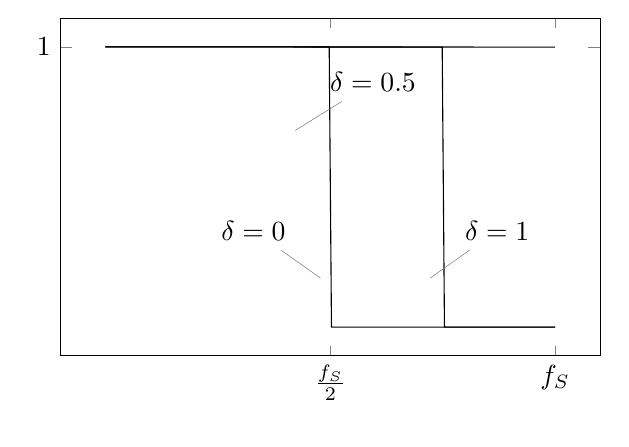
\begin{tikzpicture}
\def\fs{10}
\pgfmathparse{\fs/2}\let\fzero=\pgfmathresult
\begin{axis}[xtick={\fzero,\fs},xticklabels={$\frac{f_S}{2}$,$f_S$},ytick={1},yscale=.75,samples=200]
\foreach\delt in{0.001,0.5,1.0} {
	\pgfmathparse{(1+\delt)*\fzero}\let\band=\pgfmathresult
	\pgfmathparse{\band-\fzero}\let\fdelta=\pgfmathresult
	\pgfmathparse{\fzero-\fdelta}\let\funo=\pgfmathresult
	\addplot[domain=0:\fs]{ (abs(x)<\funo)?1.0:((abs(x)>\band)?0.0:(.5*(1+cos( (pi*(abs(x)-\funo)/(2*\fdelta)))))) };
}
\node at(axis cs:.5*\fs,0.15)[pin=135:{$\delta=0$}]{};
\node at(axis cs:.4*\fs,0.68)[pin=45:{$\delta=0.5$}]{};	
\node at(axis cs:.7*\fs,0.15)[pin=45:{$\delta=1$}]{};
\end{axis}
\end{tikzpicture}
\caption{Spettro monolatero forme d'onda di Nyquist}
\label{fig:spettro_forme_donda_Nyquist}
\end{figure}

All'aumentare del roll-off aumenta la banda e aumenta la velocità di decadimento a zero della funzione impulsiva.
Per $\delta=0$ si ha lo spettro monolatero rettangolare con banda $B=f_s/2=1/2T$, per $\delta=1$ si ha lo \keyword[spettro!a coseno rialzato]{spettro a coseno rialzato} con banda $B=f_s=\frac{1}{T}$.

Conoscendo le funzioni di trasferimento del canale di trasmissione $Q(f)$ e del filtro adattato $H(f)$ è possibile scegliere il coefficiente $\delta$ per il migliore spettro di Nyquist a coseno rialzato, $p_\text{O}(f)$.

Dato lo spettro della forma d'onda in uscita al mezzo trasmissivo $p_\text{A}(f)$ si sceglie il filtro adattato con la funzione di trasferimento $H(f)=\conj{p}_\text{A}(f)$ tale che lo spettro della forma d'onda in uscita del filtro di ricezione adattato sia $p_\text{B}(f)=\abs{p_\text{A}}^2$. Tale forma d'onda ha modulo ad intersimbolo nullo, ma è ancora possibile determinare la fase del segnale in ricezione. Ad esempio si può scegliere la fase in modo che la forma d'onda relativa abbia potenza di picco minore per evitare fenomeni di distorsione per saturazione degli amplificatori. La potenza media del segnale, che è proporzionale al modulo del segnale, non cambia.

\section{Dimensionamento}
Una volta stabilite le prestazioni desiderate da un sistema di trasmissione numerica, la quantità di informazione trasmessa per unità di tempo, il \keyword{bitrate}, e la probabilità di errore $P(\epsilon)$ massima accettabile, è necessario determinare la potenza del segnale da trasmettere.

Nel dimensionamento del sistema di trasmissione analogica si considerano fissate la banda passante del segnale da trasmettere e il rapporto segnale rumore in ricezione. Nel sistema numerico in analogia alla banda si ha la frequenza di cifra ovvero la quantità di simboli binari trasferiti al secondo, mentre la probabilità di ricevere un simbolo diverso da quello trasmesso è imputabile unicamente al disturbo sovrapposto al segnale a causa del rumore termico degli apparati di trasmissione.

Aumentare il bitrate implica aumentare la banda passante del filtro in ricezione aumentando la rumorosità del sistema causano una maggiore probabilità di errare al decisore a soglia.

Bisogna valutare la potenza da trasmettere $P_T$ mantenendo la probabilità di errore $P(\epsilon)$ inferiore al massimo tollerabile.

La probabilità di commettere un errore su un simbolo, con simboli equiprobabili, è
\begin{equation}
p(\epsilon) = p(0_T)p(1_R|0_T)+p(1_T)p(0_R|1_T) = \frac{1}{2}[p(\epsilon|0_T)+p(\epsilon|1_T)]
\end{equation}
dove le probabilità condizionate corrispondono alle aree sottese alle code delle gaussiane suddivise dal valore di soglia in fig.~\ref{fig:trasmissione_numerica_modello_statistico_decisione}
\begin{equation}
\begin{split}
p(\epsilon|0_T)&=\intd{S}{+\infty}{f_{v_C|0_T}(v)}{v}=\intd{S}{+\infty}{\frac{1}{\sqrt{2\pi}\sigma_n}\,\e{-\frac{(v-v_0)^2}{2\sigma_n^2}}}{v} \\
p(\epsilon|1_T)&=\intd{-\infty}{S}{f_{v_C|1_T}(v)}{v}=\intd{-\infty}{S}{\frac{1}{\sqrt{2\pi}\sigma_n}\,\e{-\frac{(v-v_1)^2}{2\sigma_n^2}}}{v}
\end{split}
\end{equation}
con il cambio di variabili
\[y=\frac{v-v_0}{\sigma_n}\quad \diff y=\frac{\diff v}{\sigma_n}\qquad z=\frac{v-v_1}{\sigma_n}\quad \diff z=\frac{\diff v}{\sigma_n}\]
\begin{equation}
\begin{split}
p(\epsilon|0_T)&=\intd{\frac{S-v_0}{\sigma_n}}{+\infty}{\frac{1}{\sqrt{2\pi}}\,\e{-\frac{y^2}{2}}}{y}=\f{Q}{\frac{s-v_0}{\sigma_n}} \\
p(\epsilon|1_T)&=\intd{-\infty}{\frac{S-v_1}{\sigma_n}}{\frac{1}{\sqrt{2\pi}}\,\e{-\frac{z^2}{2}}}{z}=\intd{\frac{v_1-S}{\sigma_n}}{+\infty}{\frac{1}{\sqrt{2\pi}}\,\e{-\frac{z^2}{2}}}{z}=\f{Q}{\frac{v_1-s}{\sigma_n}}
\end{split}
\end{equation}

Ponendo la soglia $s=\frac{v_0+v_1}{2}$ pari al valor medio delle tensioni corrispondenti ai picchi del segnale all'uscita dei filtri adattati si ha che le due probabilità condizionate sono 
\begin{equation}p(\epsilon|0_\text{T})=p(\epsilon|1_\text{T})=\f{Q}{\frac{v_1-v_0}{2\sigma_n}}\end{equation}

Si ha pertanto che la probabilità di errore $p(\epsilon)=\f{Q}{\gamma}$ è funzione di $\gamma=\frac{v_1-v_0}{2\sigma_n}$, ovvero proporzionale alla distanza picco picco tra i segnali di uscita dei filtri adattati e inversamente proporzionale alla deviazione standard del rumore. La funzione $\f{Q}{x}$ è l'integrale rappresentativo dell'area della coda di una gaussiana di valor medio nullo e varianza unitaria.

La varianza del rumore considerato in $\gamma$ è quella del rumore campionato. Ricordando che la densità spettrale di un processo è la trasformata di Fourier della sua funzione di autocorrelazione, segue che il rumore in uscita dal filtro adattato ha funzione di autocorrelazione
\begin{equation}
R_n^\text{B}(\tau)=\E{n^\text{B}(t)\cdot n^\text{B}(t+\tau)}
\end{equation}
che è stazionario e dipende solo dalla differenza dei tempi $\tau$.
La funzione di autocorrelazione del processo rumore campionato è
\begin{equation}
R_n^\text{C}(k T)=\E{n^\text{C}(i T)\cdot n^\text{C}(i T+k T)}
\end{equation}
Essendo il processo stazionario si ha quindi 
\begin{equation}
R_n^\text{C}(k T)=R_n^\text{B}(k T)
\end{equation}
che la funzione di autocorrelazione dei campione di rumore all'uscita del campionatore è numericamente uguale al valore della funzione di autocorrelazione del rumore prima del campionamento, presa negli istanti di tempo multipli del periodo di campionamento. Pertanto per la stazionarietà del processo rumore la varianza del rumore in uscita del campionatore è 
\begin{equation}
\restrict{\sigma^2_n}{\text{C}}=R_n^\text{C}(0)=R_n^\text{B}(0)
\end{equation}
Per la ergodicità del processo si ha anche che la varianza è pari alla potenza media del rumore all'uscita del filtro di ricezione 
\begin{equation}
\restrict{\sigma^2_n}{\text{C}}=P_{n \text{medio}}^\text{B}
\end{equation}

Nell'ipotesi di \keyword[codifica!antipodale]{codifica antipodale} si ha a valle del campionatore l'uscita dei filtri adattati con la massima distanza tra le tensioni $v_0=-a$ e $v_1=+a$ con la soglia posta a $s=0$ e il valore $\gamma=a/\sigma$. A monte del campionatore alla tensione di picco $v_\text{picco}=\pm a$ corrisponde una potenza pari al quadrato della tensione (ipotizzando una impedenza unitaria).
\begin{equation}
\restrict{\frac{S}{N}}{B}=\gamma^2=\frac{a^2}{\sigma_n^2}=\frac{P_\text{S picco}^\text{B}}{P_\text{N media}^\text{B}}
\label{eq:rapporto_segnale_rumore_uscita_filtro_adattato}
\end{equation}

Il massimo rapporto segnale rumore all'uscita del filtro adattato è esprimibile in funzione dei parametri all'ingresso del filtro come rapporto tra l'energia della forma d'onda che rappresenta il simbolo ricevuto e la densità spettrale bilatera della potenza di rumore all'uscita del canale
\begin{equation}
\restrict{\frac{S}{N}}{B}=\frac{E_\text{R}}{h_n^\text{A}/2}=\frac{E_\text{R}/T}{h_n^\text{A}/2\cdot f_\text{S}}=\frac{P_\text{S media}^\text{A}}{h_n^\text{A} f_\text{S}/2}
\end{equation}

Si ottiene che il rapporto segnale rumore è al numeratore la potenza media del segnale ricevuto, a denominatore la potenza media del rumore all'ingresso misurata rapportata alla banda $f_\text{S}/2$.

Nell'ipotesi di \keyword[codifica!ortogonale]{codifica ortogonale} si ha a valle del campionatore l'uscita dei filtri adattati con la distanza tra le tensioni $v_0=0$ e $v_1=+a$ con la soglia posta a $s=a/2$ e il valore $\gamma=a/2\sigma$. 
\begin{equation}
\restrict{\frac{S}{N}}{B}=\gamma^2=\frac{a^2}{4\sigma_n^2}=\frac{P_\text{S picco}^\text{B}}{4 P_\text{N media}^\text{B}}=\frac{E_\text{R}}{4 h_n^\text{A}/2}=\frac{E_\text{R}/T}{2 h_n^\text{A}\cdot f_\text{S}}=\frac{P_\text{S media}^\text{A}}{h_n^\text{A} f_\text{S}}
\end{equation}
dove $E_R$ è l'energia ricevuta quando c'è la forma d'onda del simbolo “1”, pertanto $E_R/T$ rappresenta il doppio della potenza media del segnale ricevuto.

Dal confronto tra i rapporti segnale rumore della codifica ortogonale e codifica antipodale si evince che per ottenere da un sistema con condifica ortogonale la stessa probabilità di errore che si ottiene con codifica ortogonale, è necessario trasmettere una potenza media doppia, ovvero $\SI{3}{\decibel}$ superiore.

\begin{esercizio}
	Si voglia \textsc{progettare un sistema di trasmissione numerica digitale multitratta} con una velocità $\SI{100}{\mega\bit\per\second}$ con una probabilità di errore non superiore a $p(\epsilon)=\num{e-7}$ su un cavo di lunghezza $L=\SI{100}{\kilo\meter}$ che attenuazione specifica $\alpha_\text{sp}=\SI{1}{\decibel\per\kilo\meter}$ alla frequenza $f_\text{sp}=\SI{1}{\mega\hertz}$, con equalizzazione passiva e codifica antipodale.
\end{esercizio}

\`{E} necessario calcolare il rapporto segnale rumore all'uscita del campionatore che garantisca $p(\epsilon)=\num{e-7}$. Ipotizzando un rumore gaussiano bianco sovrapposto al segnale e una soglia nel valor medio delle tensioni all'uscita del filtro adattato si ha $p(\epsilon)=\f{Q}{\gamma}$. Ricordando mnemonicamente che per $p(\epsilon)=\num{e-6}$ si ha un valore di $\gamma=\SI{13.5}{\decibel}$ e che per diminuire di un fattore 10 la probabilità di errore è necessario aumentare $\gamma$ di un $\SI{1}{\decibel}$ si ha che per $p(\epsilon)=\num{e-7}$ si ottiene $\gamma=\SI{14.5}{\decibel}$.

Nell'ipotesi di codifica antipodale il rapporto all'uscita del filtro di ricezione della potenza di picco del segnale e la potenza media di rumore
\[\gamma^2=\frac{P_\text{S picco}^\text{B}}{P_\text{N media}^\text{B}}=\SI{14.5}{\decibel}\]
Nell'ipotesi di utilizzare un filtro adattato, sempre in codifica antipodale, si ha che il rapporto segnale rumore risulta pari a 
\[\frac{P_\text{S media}^\text{A}}{\frac{h_n^\text{A}}{2} f_\text{S}}=\SI{14.5}{\decibel}\]

Nota la rumorosità delle apparecchiature riceventi, per ipotesi un fattore di rumore $F=\SI{10}{\decibel}$, si può valutare la minima potenza media necessaria in ricezione per rispettare i requisiti di progetto (espressa in $\si{\dBm}$):
\[P_\text{S media}^\text{A}=\restrict{\gamma^2}{\si{\decibel}}+\restrict{h_n}{\si{\decibel}}+\restrict{F}{\si{\decibel}}+\restrict{\frac{f_s}{2}}{\si{\decibel}}=(\num{14.5}-174+10+77)\si{\dBm}=\SI{-72.5}{\dBm}\]

Nell'ipotesi di equalizzazione passiva si calcola l'attenuazione totale $\alpha_\text{TOT}$ determinando l'attenuazione specifica alla frequenza massima del segnale, che per forma d'onda di Nyquist con coefficiente di roll-off $\delta=1$ è $f_\text{max}=\frac{1}{T}=\SI{100}{\mega\hertz}$:
\[\alpha_{f_\text{max}}=\alpha_\text{rif}\sqrt{\frac{f_\text{max}}{f_\text{rif}}}=\SI{1}{\decibel\per\kilo\meter}\cdot\sqrt{\frac{\num{100e6}}{\num{e6}}}=\SI{10}{\decibel\per\kilo\meter}\to \alpha_\text{TOT}=L\cdot\alpha_{f_\text{max}}=\SI{1000}{\decibel}\]

Tale attenuazione è eccessiva per una trasmissione su una unica tratta. Si deve ricorrere ad un sistema multitratta analogico, dividendo la lunghezza del cavo in più sezioni e ritrasmettendo il segnale con apparecchiature di amplificazione.

Ipotizzando che ogni trasmettitore abbia una potenza massima di trasmissione pari a $P_T=\SI{100}{\milli\watt}$, che le tratte siano tutte uguali e che all'uscita dell'ultima tratta si voglia ottenere un rapporto segnale rumore $\restrict{S/N}{u}=\SI{14.5}{\decibel}$ si calcoli il numero di tratte.

L'attenuazione sulla singola tratta sarà $\alpha_\text{tot}/n$, mentre il rumore risulta moltiplicato per $n$: il rumore della prima tratta viene amplificato/attenuato e iniettato nella seconda tratta, e così via.

Sempre in ipotesi di codifica antipodale si ha che il rapporto segnale rumore è pari a 
\[\gamma^2=\frac{P_\text{S medio}^\text{B}}{P_\text{N}^\text{B}}=\frac{P_T\cdot\alpha_\text{tot}/n}{n\cdot\frac{h_n}{2}f_s}\]

\[\restrict{\gamma^2}{\si{\decibel}}\leq \restrict{P_T}{\si{\dBm}} - \restrict{\frac{\alpha_\text{tot}}{n}}{\si{\decibel}}-10\Log{n}-\restrict{F\frac{h_n f_s}{2}}{\si{\dBm}}\]

\[ \SI{14.5}{\decibel}\leq\SI{20}{\dBm} - \frac{\SI{1000}{\decibel}}{n}-10\Log{n}-(-\SI{174}{\dBm}+\SI{10}{\decibel}-\SI{3}{\decibel}+\SI{80}{\decibel})\]

Espressione che ha soluzione per $n\geq 13$.

\begin{figure}[ht!]\centering
\subfloat[Multitratta analogico]{
	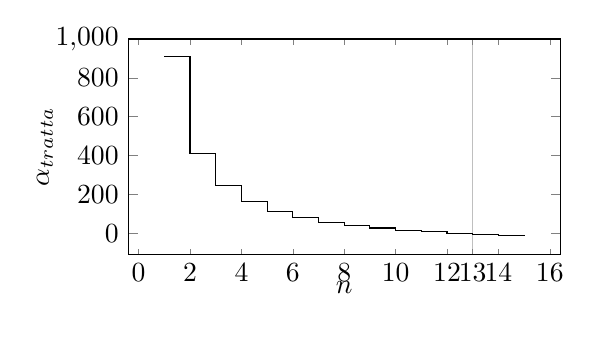
\begin{tikzpicture}[scale=.8]
	\begin{axis}[yscale=.6,xlabel=$n$,ylabel=$\alpha_\text{tratta}$,samples at={1,...,15},extra x ticks={13},
	extra x tick style={grid=major}]
	\addplot[const plot]{14.5+10*log10(x)-20+1000/x-87};
	\end{axis}
	\end{tikzpicture}}\quad%
\subfloat[Multitratta digitale]{
	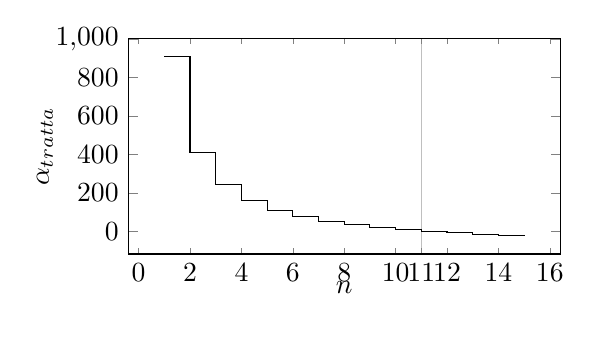
\begin{tikzpicture}[scale=.8]
	\begin{axis}[yscale=.6,xlabel=$n$,ylabel=$\alpha_\text{tratta}$,samples at={1,...,15},extra x ticks={11},
	extra x tick style={grid=major}]
	\addplot[const plot]{14.5+log10(x)-20+1000/x-87};
	\end{axis}
	\end{tikzpicture}}
\end{figure}

In alternativa al sistema multitratta analogico che ha il difetto di moltiplicare $n$ volte il rumore in uscita è possibile adottare il multitratta digitale in cui si rigenera il segnale numerico alla fine di ogni tratta. Ogni tratta è un sistema di trasmissione numerico a sé stante, non trasferisce il rumore da una tratta all'altra, è caratterizzato dalla propria probabilità di errore statisticamente indipendente dalle altre tratte, pertanto il numero medio di bit errati sarà la somma dei bit errati su ogni tratta. Si ha così che la probabilità di errore complessiva è pari alla somma delle probabilità di errore sulle singole tratte
\begin{equation}
P_\text{tot}(\epsilon)=\sum_{i}p_i(\epsilon)
\end{equation}

La probabilità di errore finale, con tratte uguali, è
\begin{equation}
p(\epsilon)=1-\prod_{i=1}^{n}[1-p_i(\epsilon)]=1-[1-p_\text{ST}(\epsilon)]^n\cong 1-[1-n\cdot p_\text{ST}(\epsilon)]\cong n\cdot p_\text{ST}(\epsilon)
\end{equation}

Se il sistema di trasmissione numerico deve garantire una probabilità di errore $p(\epsilon)$, ad esempio di $p(\epsilon)\leq\num{e-7}$, il dimensionamento di un sistema multitratta digitale richiede che ogni singola tratta abbia una probabilità di errore $n$ volte più piccola:
\begin{equation}p_\text{ST}(\epsilon)\leq\frac{p(\epsilon)}{n}\end{equation}

Nel caso di studio in esame il dimensionamento richiede che il rapporto segnale rumore sia superiore a $\restrict{\gamma^2}{\si{\decibel}}=\SI{14.5}{\decibel}+\Log{N}$. La correzione si ha perché se ad ogni $p(\epsilon)/10$ corrisponde un aumento del rapporto segnale rumore di $\SI{1}{\decibel}=10\Log{10}$, ad un errore per tratta $p(\epsilon)/n$ corrisponde un aumento di $\Log{n}\si{\decibel}$.

\[P_T-\frac{\alpha_\text{tot}}{n}-F\frac{h_n f_s}{2}\geq \num{14.5}+\Log{n}\]

\section{Estrazione del timing}
Il campionatore deve effettuare il campionamento del segnale all'uscita del filtro di ricezione quando questo raggiunge il suo valore massimo per massimizzare il rapporto segnale rumore in B pari al valore $\gamma^2$ (eq.~\ref{eq:rapporto_segnale_rumore_uscita_filtro_adattato}). Non è possibile utilizzare un oscillatore che comandi il campionatore e che oscilli esattamente alla frequenza desiderata pari a quella del trasmettitore, anche piccoli errori nel periodo sfaserebbero i circuiti, inoltre è impossibile conoscere la fase corretta a causa del ritardo di propagazione lungo il mezzo trasmissivo. L'unico modo per sincronizzare il campionatore è quello di ricavare il timing estraendo l'informazione dalla fase e la frequenza dello stesso segnale ricevuto.
\begin{figure}[!ht]
	\centering
	\resizebox{\textwidth}{!}{
		\begin{tikzpicture}[>=latex']
		\coordinate(c0);
		\node[block,right=1.5cm of c0](b0){GFO};
		\node[block,right=1.5cm of b0](b1){MT};
		\node[sum,right=1cm of b1](s0){$+$};
		\coordinate[above=1cm of s0](n);
		\coordinate[right=1cm of s0](n1);
		\node[block,right=1cm of n1](b2){FR};
		\node[block,below=1cm of b2](b4){TIMING};
		\node[campionatore,right=1cm of b2](q0){};
		\node[block,right=1cm of q0](b3){DEC};
		\coordinate[right=1.5cm of b3](c1);
		\draw[->](c0)--node[above,near start]{bit}(b0);
		\draw[dot=O](b0)--(b1);
		\draw[->](b1)--(s0);
		\draw[->](n)node[above]{$n(t)$}--(s0);
		\draw[->](n1)|-(b4);
		\draw[->](b4)-|(q0);
		\draw[->](s0)--(b2);
		\draw[dot=B](b2)--(q0);
		\draw[dot=C](q0)--(b3);
		\draw[->](b3)--node[above,near end]{bit}(c1);
		\node[fitted, fit=(b0),label=above:Trasmettitore]{};
		\node[fitted, fit=(b1)(s0),label=above:Canale]{};
		\node[fitted, fit=(b2)(q0)(b3)(b4),label=above:Ricevitore]{};
		\end{tikzpicture}
	}
	\caption{Schema sistema di trasmissione numerico con estrattore del timing}
	\label{fig:schema_sistema_trasmissione_numerico_timing}
\end{figure}

Nell'ipotesi di utilizzare forme d'onda rettangolari di periodo di cifra $T$, una sequenza di $a\rect{t/T}$ ritardati, non è possibile utilizzare un filtro passa banda molto stretta attorno alla frequenza di cifra $f_S=1/T$, essendo nullo il contributo spettrale del $a T\sinc{f T}$ in corrispondenza di tale frequenza e sue armoniche, alla quale si trova solo rumore.

Si studia come poter alterare le sequenze di impulsi rettangolari per codificare nel segnale trasmesso l'informazione di temporizzazione con i \keyword[codice di linea]{codici di linea}.

\section{Codici di linea}
\subsection{Codice \ac{NRZ}}
Una sequenza di impulsi rettangolari che mantengono costante il proprio valore nel periodo $T$. In caso di simboli ripetuti il segnale \keyword[codifica!NRZ]{non ritorna a zero} mantenendo il livello alto. Il contenuto spettrale alla frequenza $1/T$ è praticamente nullo.
L'informazione sulla temporizzazione è contenuta nei fronti di salita e discesa del segnale: per recuperare il timing è necessario derivare il segnale, raddrizzarlo e filtrare passa banda stretta sulla frequenza di cifra $1/T$ per estrarre gli impulsi di pilotaggio per il campionatore. Si ottiene un treno di impulsi quasi periodico: una lunga sequenza di “0” o “1” fa perdere il sincronismo.

\begin{figure}[ht!]
\centering
\subfloat[Codice \ac{NRZ} ortogonale]{
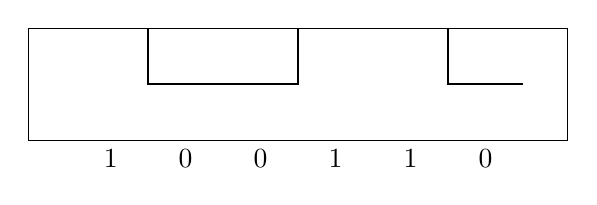
\begin{tikzpicture}
	\begin{axis}[xtick=\empty,ytick=\empty,yscale=.25,every extra x tick/.append style={major tick length=0pt},extra x ticks={.5,1.5,2.5,3.5,4.5,5.5},extra x tick labels={1,0,0,1,1,0},ymin=-1,ymax=1]
	\addplot [const plot,thick,draw=black]coordinates {(0,1)(1,0)(2,0)(3,1)(5,0)(6,0)};
	\end{axis}
\end{tikzpicture}}%
\subfloat[Impulsi di temporizzazione \ac{NRZ} ortogonale]{
	\begin{tikzpicture}
	\begin{axis}[xtick=\empty,ytick=\empty,yscale=.25]
	\addplot [quiver={u=0,v=1},-latex']coordinates {(0,0)(1,0)(3,0)(5,0)};
	\addplot [quiver={u=0,v=-1},-latex',dotted,gray]coordinates {(1,0)(5,0)};
	\end{axis}
	\end{tikzpicture}}

\subfloat[Codice \ac{NRZ} antipodale]{
	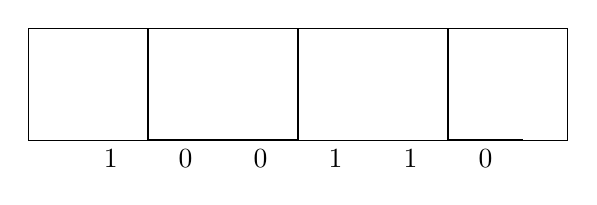
\begin{tikzpicture}
	\begin{axis}[xtick=\empty,ytick=\empty,yscale=.25,every extra x tick/.append style={major tick length=0pt},extra x ticks={.5,1.5,2.5,3.5,4.5,5.5},extra x tick labels={1,0,0,1,1,0},ymin=-1,ymax=1]
	\addplot [const plot,thick,draw=black]coordinates {(0,1)(1,-1)(2,-1)(3,1)(5,-1)(6,-1)};
	\end{axis}
	\end{tikzpicture}}%
\subfloat[Impulsi di temporizzazione \ac{NRZ} antipodale]{
	\begin{tikzpicture}
	\begin{axis}[xtick=\empty,ytick=\empty,yscale=.25]
	\addplot [quiver={u=0,v=1},-latex']coordinates {(0,0)(1,0)(3,0)(5,0)};
	\addplot [quiver={u=0,v=-1},-latex',dotted,gray]coordinates {(1,0)(5,0)};
	\end{axis}
	\end{tikzpicture}}%
\end{figure}

\subsection{Codice \ac{RZ}}
Una sequenza di impulsi rettangolari con codifica \ac{RZ} a valore costante di durata $\tau<T$. A parità di potenza di picco la potenza media del segnale con \keyword[codifica!RZ]{ritorno a zero} è inferiore a quella senza ritorno a zero (e rispetto al rumore). Lo spettro della forma d'onda è dato dalla sovrapposizione degli impulsi $a\tau\frac{sin{\pi f\tau}}{\pi f\tau}\e{-\jmath 2\pi f k\tau}$ che danno un contributo non nullo alla frequenza $1/T$, pari a $a\tau\frac{sin{\pi\tau/T}}{\pi\tau/T}$, consentendo l'estrazione del timing con un filtro molto stretto accordato alla frequenza $1/T$.

Utilizzando una codifica antipodale associando valori di tensione opposti alle forme d'onda che codificano i simboli si può ottenere dal circuito derivatore e raddrizzatore un maggior numero di impulsi di pilotaggio per il campionatore per una migliore temporizzazione.

\begin{figure}[ht!]
	\centering
	\subfloat[Codifica \ac{RZ} ortogonale]{
		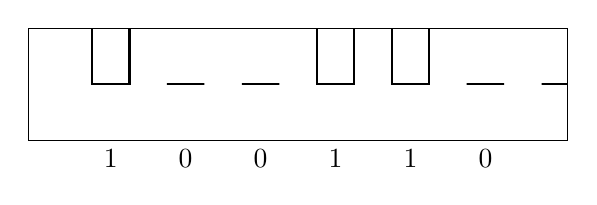
\begin{tikzpicture}
		\begin{axis}[ybar,bar shift=.5,bar width=.5,xtick=\empty,ytick=\empty,yscale=.25,every extra x tick/.append style={major tick length=0pt},extra x ticks={0.5,1.5,2.5,3.5,4.5,5.5},extra x tick labels={1,0,0,1,1,0},ymin=-1,ymax=1]
		\addplot [thick,draw=black]coordinates {(0,1)(1,0)(2,0)(3,1)(4,1)(5,0)(6,0)};
		\end{axis}
		\end{tikzpicture}}
	\subfloat[Impulsi di temporizzazione \ac{RZ} ortogonale]{
		\begin{tikzpicture}
		\begin{axis}[xtick=\empty,ytick=\empty,yscale=.25,ymin=-1,ymax=1]
		\addplot [quiver={u=0,v=1},-latex']coordinates {(0.25,0)(.75,0)(3.25,0)(3.75,0)(5.25,0)(5.75,0)};
		\addplot [quiver={u=0,v=-1},-latex',dotted,gray]coordinates {(.75,0)(3.75,0)(5.75,0)};
		\end{axis}
		\end{tikzpicture}}
	
	\subfloat[Codifica \ac{RZ} antipodale]{
		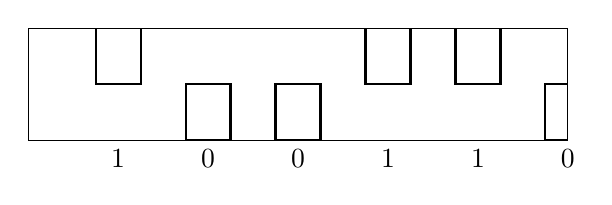
\begin{tikzpicture}
		\begin{axis}[ybar,bar shift=.5,bar width=.5,xtick=\empty,ytick=\empty,yscale=.25,every extra x tick/.append style={major tick length=0pt},extra x ticks={0.5,1.5,2.5,3.5,4.5,5.5},extra x tick labels={1,0,0,1,1,0},ymin=-1,ymax=1]
		\addplot [thick,draw=black]coordinates {(0,1)(1,-1)(2,-1)(3,1)(4,1)(5,-1)};
		\end{axis}
		\end{tikzpicture}}
	\subfloat[Impulsi di temporizzazione \ac{RZ} antipodale]{
		\begin{tikzpicture}
		\begin{axis}[xtick=\empty,ytick=\empty,yscale=.25,ymin=-1,ymax=1]
		\addplot [quiver={u=0,v=1},-latex']coordinates {(0.25,0)(.75,0)(1.25,0)(1.75,0)(2.25,0)(2.75,0)(3.25,0)(3.75,0)(4.25,0)(4.75,0)(5.25,0)(5.75,0)};
		\addplot [quiver={u=0,v=-1},-latex',dotted,gray]coordinates {(.75,0)(1.25,0)(2.25,0)(3.75,0)(4.75,0)(5.25,0)};
		\end{axis}
		\end{tikzpicture}}%
\end{figure}

\subsection{Codice \ac{AMI}}
Una alternativa alla codifica con ritorno a zero che causa una perdita di energia del segnale per ottenere una migliore estrazione di segnale di temporizzazione è l'utilizzo del codice di linea \ac{AMI} di tipo non ritorno a zero con codifica ortogonale con i simboli “1” realizzati alternativamente con impulsi di tensione $\pm 1$. La sequenza ripetuta di simboli “1” darà luogo a discontinuità che saranno rilevate dal derivatore, incrementando il numero di impulsi al raddrizzatore. Lo spettro di potenza ha valor medio nullo e il segnale non ha informazione in componente continua consentendo l'utilizzo della codifica per apparati alimentati a distanza.

\begin{figure}[ht!]\centering
\subfloat[Codifica \ac{AMI}]{
	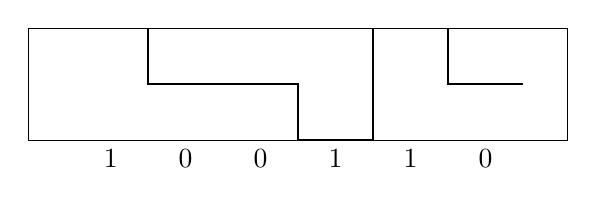
\begin{tikzpicture}
		\begin{axis}[xtick=\empty,ytick=\empty,yscale=.25,every extra x tick/.append style={major tick length=0pt},extra x ticks={.5,1.5,2.5,3.5,4.5,5.5},extra x tick labels={1,0,0,1,1,0},ymin=-1,ymax=1]
		\addplot [const plot,thick,draw=black]coordinates {(0,1)(1,0)(2,0)(3,-1)(4,1)(5,0)(6,0)};
		\end{axis}
	\end{tikzpicture}}
\subfloat[Impulsi di temporizzazione \ac{AMI}]{
	\begin{tikzpicture}
	\begin{axis}[xtick=\empty,ytick=\empty,yscale=.25,ymin=-1,ymax=1]
	\addplot [quiver={u=0,v=1},-latex']coordinates {(0,0)(1,0)(3,0)(4,0)(5,0)};
	\addplot [quiver={u=0,v=-1},-latex',dotted,gray]coordinates {(1,0)(3,0)(5,0)};
	\end{axis}
	\end{tikzpicture}}%
\end{figure}

\subsection{Codice \ac{HDB-3}}
Per risolvere l'analogo problema relativo alla trasmissione di più simboli “0” consecutivi si introduce il codice \ac{HDB-3} come evoluzione del codice \ac{AMI}: per evitare che non arrivino impulsi al circuito di estrazione del timing per più di 3 periodi di cifra in corrispondenza di un quarto zero consecutivo si invia un impulso rettangolare con la stessa tensione dell'“1” precedente. Violando l'alternanza del codice \ac{AMI} il simbolo sarà interpretato non come un “1” ma come uno “0”. 

\begin{figure}[ht!]\centering
	\subfloat[Codifica \ac{HDB-3}]{
		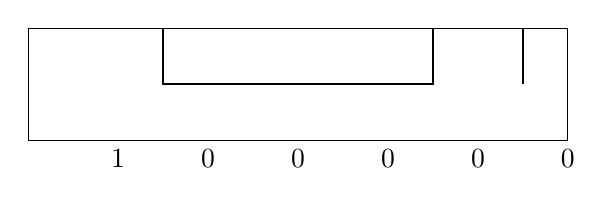
\begin{tikzpicture}
		\begin{axis}[xtick=\empty,ytick=\empty,yscale=.25,every extra x tick/.append style={major tick length=0pt},extra x ticks={.5,1.5,2.5,3.5,4.5,5.5},extra x tick labels={1,0,0,0,0,0},ymin=-1,ymax=1]
		\addplot [const plot,thick,draw=black]coordinates {(0,1)(1,0)(2,0)(3,0)(4,1)(5,0)};
		\end{axis}
		\end{tikzpicture}}
	\subfloat[Impulsi di temporizzazione \ac{HDB-3}]{
		\begin{tikzpicture}
		\begin{axis}[xtick=\empty,ytick=\empty,yscale=.25,ymin=-1,ymax=1]
		\addplot [quiver={u=0,v=1},-latex']coordinates {(0,0)(1,0)(4,0)(5,0)};
		\addplot [quiver={u=0,v=-1},-latex',dotted,gray]coordinates {(1,0)(5,0)};
		\end{axis}
		\end{tikzpicture}}%
\end{figure}

\subsection{Codice Manchester}
Il \keyword[codice di linea!Manchester]{codice Manchester} garantisce per entrambe i simboli la transizione in salita o discesa a metà periodo: questo garantisce la presenza dell'impulso di sincronizzazione per la migliore temporizzazione pur dimezzando la potenza media del segnale.


\begin{figure}[ht!]
	\centering
	\subfloat[Codice Manchester]{
		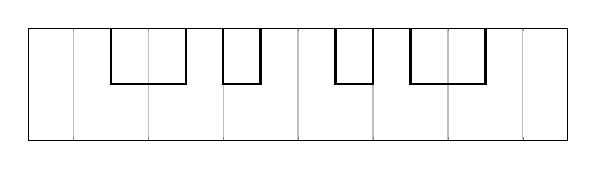
\begin{tikzpicture}
		\begin{axis}[xticklabels={},xmajorgrids,ytick=\empty,yscale=.25,ymin=-1,ymax=1]
		\addplot [const plot,thick,draw=black]coordinates {(0,1)(.5,0)(1,0)(1.5,1)(2,0)(2.5,1)(3,1)(3.5,0)(4,1)(4.5,0)(5,0)(5.5,1)(6,1)};
%		\foreach\bit[count=\ii]in{1,0,0,1,1,0}{\node at(axis cs:\ii,0){\bit};};
		\end{axis}
		\end{tikzpicture}}
	\subfloat[Impulsi di temporizzazione con codice Manchester]{
		\begin{tikzpicture}
		\begin{axis}[ytick=\empty,yscale=.25,ymin=-1,ymax=1]
		\addplot [quiver={u=0,v=1},-latex']coordinates {(0.5,0)(1.5,0)(2.5,0)(3.5,0)(4.5,0)(5.5,0)};
		\end{axis}
		\end{tikzpicture}}
\end{figure}

\clearpage
\section{Rinuncia al filtraggio adattato}\label{cap:rinuncia_filtro_adattato}
Il dimensionamento di un sistema di trasmissione numerico deve massimizzare il rapporto segnale rumore al campionatore a parità di potenza media ricevuta
\[\restrict{\frac{S}{N}}{C}=\frac{E_R}{h_n/2}\]

La progettazione di un sistema di trasmissione numerica basato su forme d'onda di Nyquist e filtro adattato massimizza il rapporto segnale rumore al campionatore perché si campiona il segnale nel suo picco ottenuto con un integratore ad azzeramento. La potenza di picco è proporzionale al quadrato dell'ampiezza massima del segnale campionato. Per la necessità di avere forme d'onda ad intersimbolo nullo all'uscita del filtro si scelgono segnali della famiglia di Nyquist, e il modulo dello spettro del segnale è legato al coefficiente di roll-off. La fase viene scelta in modo tale da ovviare alle limitazioni sulla potenza di picco dovute ai limiti di saturazione degli amplificatori. 
Un sistema di trasmissione basato su filtro adattato è fortemente vulnerabile ad ogni distorsione delle forme d'onda produce una riduzione del rapporto segnale rumore $\restrict{S/N}{C}$.

\begin{figure}[!ht]
	\centering
		\begin{tikzpicture}[>=latex']
		\coordinate(start);
		\node[block,right=1.5cm of start](ht){$H_T(f)$};
		\draw[->](start)--node[below,near start]{$S_T^\text{O}(f)$}(ht);
		\node[sum,right=1cm of ht](s0){$+$};
		\draw[dot=A](ht)--(s0);
		\coordinate[above=1cm of s0](n);
		\draw[->](n)node[above]{$n(t)$}--(s0);
		\node[block,right=1cm of s0](hr){$H_R(f)$};
		\draw[->](s0)--(hr);
		\node[campionatore,right=1cm of hr](q0){};
		\coordinate[right=1.5cm of q0](end);
		\draw[dot=B](hr)--(q0);
		\draw[dot=C](q0)--(end);
		\node[fitted, fit=(ht)(s0),label=above:Canale]{};
		\node[fitted, fit=(hr)(q0),label=above:Ricevitore]{};
		\end{tikzpicture}
	\caption{Schema filtro di ricezione}
	\label{fig:schema_filtro_ricezione}
\end{figure}

Per superare i limiti di tale sistema di trasmissione si rinuncia al filtro adattato che vincola la potenza media trasmessa e si ottimizzano le prestazioni utilizzando forme d'onda rettangolari in trasmissione che presentano la massima efficienza avendo la potenza media pari alla potenza di picco. 

Impulsi rettangolari di ampiezza $a$ e durata $\tau\leq T$ (con $\tau<T$ si ha codifica con ritorno a zero per facilitare il sincronismo) hanno espressione nel tempo e in frequenza, al trasmettitore:
\begin{equation}
\begin{split}
s_T^\text{O}(t)&=a\rect{\frac{t}{\tau}}\\
S_T^\text{O}(f)&=a\tau\frac{\sen{\pi f\tau}}{\pi f\tau}
\end{split}
\end{equation}

Si valuta il rapporto segnale rumore al campionatore del segnale ricevuto 
\begin{equation}
\restrict{\frac{S}{N}}{C}=\frac{P_\text{S picco}}{P_\text{N media}}
\end{equation}
e si confronta il risultato con quello ottenuto con il filtro adattato.

Date le funzioni di trasferimento del canale $H_T(f)$, del filtro generico $H_R(f)$, valutando la potenza del segnale nell'istante $t_m$ di picco, indicando con $h_n$ la densità spettrale monolatera di rumore bianco, valutando la potenza media di rumore a valle del filtro, si ha
\begin{equation}
\begin{split}
\restrict{\frac{S}{N}}{C}&=\frac{\abs{\intinf{ S_T(f) H_T(f)H_R(f)\e{\jmath 2\pi f t_m}}{f}}^2}{\intinf{\frac{h_n}{2}\abs{H_R(f)}^2}{f}}=\\
&=\frac{\abs{\intinf{ a\tau \frac{\sen{\pi f\tau}}{\pi f\tau} H_T(f)H_R(f)\e{\jmath 2\pi f t_m}}{f}}^2}{\frac{h_n}{2}\intinf{\abs{H_R(f)}^2}{f}}=\\
&=\frac{a^2}{\frac{h_n}{2}f_s}\underbrace{\frac{\tau^2}{T}\frac{\abs{\intinf{\frac{\sen{\pi f\tau}}{\pi f\tau} H_T(f)H_R(f)\e{\jmath 2\pi f t_m}}{f}}^2}{\intinf{\abs{H_R(f)}^2}{f}}}_{\text{rapporto adimensionale}}=\\
&=\frac{a^2}{\frac{h_n}{2}f_s}\e{-2\alpha_e}
\end{split}
\end{equation}

Si ottiene che il rapporto segnale rumore al campionatore è proporzionale alla potenza di picco del segnale trasmesso, dove essendo $a^2$ il quadrato dell'ampiezza del rettangolo trasmesso, affetto da una attenuazione esponenziale equivalente pari al rapporto adimensionale tra gli integrali. Tale rapporto dipende dalla forma d'onda trasmessa, dato dalla durata del rettangolo $\tau$ rispetto al periodo di cifra $T$, dal roll-off se tale forma d'onda appartiene alla famiglia di Nyquist, e dalle caratteristiche del mezzo trasmissivo.

Per confrontare il risultato con il rapporto segnale rumore ottenuto con filtro adattato che è pari a \[\restrict{\frac{S}{N}}{C}=\frac{P_\text{R media}}{\frac{h_n}{2}f_s}\]
è necessario valutare l'espressione dell'attenuazione equivalente essendo, nel caso di codifica \ac{NRZ}, con $\tau=T$ la potenza di picco pari alla potenza media trasmessa. 

Si deve progettare il filtro ipotizzando di dover equalizzare gli effetti di attenuazione di un mezzo di trasmissione ideale, con funzione di trasferimento $H_T(f)=\e{-\alpha_T}$, con $\alpha_T$ costante, e imponendo che l'impulso rettangolare in ricezione all'uscita del filtro abbia una forma d'onda di Nyquist per ottenere l'intersimbolo nullo:
\begin{equation}
a\tau S_R^\text{B}(f)=a\tau\frac{\sen{\pi f\tau}}{\pi f\tau} H_T(f) H_R(f)
\end{equation}
da cui si ricava, potendo invertire lo spettro della forma d'onda di Nyquist che non si annulla nelle frequenze $f\in[0,f_s]$,
\begin{equation}
H_R(f)=S_R^\text{B}(f) H_T^{-1}(f) \frac{\pi f\tau}{\sen{\pi f\tau}}
\end{equation}
Sostituendo tale risultato nel rapporto adimensionale tra integrali si ottiene che il rapporto segnale rumore ha espressione:
\begin{equation}
\begin{split}
\restrict{\frac{S}{N}}{C}&=\frac{a^2}{\frac{h_n}{2}f_s} \frac{\tau^2}{T}\frac{\abs{\intinf{S_R^\text{B}(f)\e{\jmath 2\pi f t_m}}{f}}^2}{\intinf{\abs{S_R^\text{B}(f) \e{\alpha_T}\frac{\pi f\tau}{\sen{\pi f\tau}}}^2}{f}}=\\
&=\frac{a^2}{\frac{h_n}{2}f_s}\e{-2\alpha_T}\e{-2\alpha_F}
\end{split}
\end{equation}
Avendo espresso il fattore di attenuazione del mezzo trasmissivo ideale nel restante fattore adimensionale confluisce l'attenuazione $\e{\alpha_F}$ dovuta al \keyword[fattore di forma]{fattore di forma} che dipende dalle forme d'onda trasmesse. A numeratore si ha quindi la potenza di picco ricevuta:
\begin{equation}
\restrict{\frac{S}{N}}{C}=\frac{P_\text{R picco}^\text{A}}{\frac{h_n}{2}f_s}\e{-2\alpha_F}
\end{equation}
Per codifiche di non ritorno a zero con $\tau=T$ si la potenza di picco in ricezione coincide con la potenza media ricevuta $P_\text{R picco}^\text{A}=P_\text{R media}^\text{A}$ pertanto
\begin{equation}
\restrict{\frac{S}{N}}{C}=\frac{P_\text{R media}^\text{A}}{\frac{h_n}{2}f_s}\e{-2\alpha_F}
\end{equation}
La formula con il filtro adattato ha rapporto segnale rumore 
\begin{equation}
\restrict{\frac{S}{N}}{C}=\frac{P_\text{R media}^\text{A}}{\frac{h_n}{2}f_s}
\end{equation}

In un bilancio di potenze l'entità dell'attenuazione data dal fattore di forma vale circa $\SI{0.5}{\decibel}$ ma il guadagno in termini di efficienza dell'amplificatore in trasmissione dell'ordine anche di $\SI{10}{\decibel}$ di potenza trasmessa (trasmettendo rettangoli si possono mandare gli amplificatori in saturazione).

Tale risultato continua a valere anche nel caso di mezzo trasmissivo non ideale: è necessario che l'attenuazione $\alpha_T$ sia costante solo nella banda di frequenze dello spettro del segnale all'uscita del filtro di ricezione ovvero delle forme d'onda di Nyquist, per le quali la frequenza massima è data da eq.\ref{eq:banda_nyquist} $B=(1+\delta)f_s/2$.

Nel dimensionamento di un sistema di trasmissione numerico con filtro generico, data una probabilità di errore tollerabile, si vuole determinare l'ampiezza del segnale rettangolare da trasmettere, ricordando che $\gamma=a/\sigma$ per codifica antipodale e $\gamma=a/2\sigma$ per codifica ortogonale, si impone che 
\begin{equation}
\frac{P_\text{T picco}^\text{A}}{\frac{h_n}{2}f_s}=\gamma^2\e{2\alpha_e}
\end{equation}
L'attenuazione equivalente $\alpha_e$ può essere calcolata integrando numericamente la funzione di trasferimento del mezzo trasmissivo. Nel caso di mezzo trasmissivo ideale con attenuazione costante $\alpha_T$ almeno nella banda delle forme d'onda di Nyquist, si impone che 
\begin{equation}
\frac{P_\text{R media}^\text{A}}{\frac{h_n}{2}f_s}=\gamma^2\e{2\alpha_F}
\end{equation}
Una volta calcolata l'ampiezza del segnale da trasmettere è possibile determinare la funzione di trasferimento del filtro di ricezione.

\section{Effetto di disturbi generici}
Si è visto come per evitare l'interferenza intersimbolica si imponga di ricevere all'uscita del filtro in ricezione delle forme d'onda di Nyquist a zeri equidistanti. L'effetto di errori di campionamento viene mitigato dall'ampiezza limitata della forma d'onda che si ottiene per roll-off maggiori di $\delta>0$ (idealmente $\delta=1$) al prezzo di un maggior utilizzo di banda e maggior potenza di rumore passante dal filtro.

Si valuta ora l'effetto di disturbi generici di altra natura rispetto al rumore termico gaussiano bianco. Le potenze medie dei segnali di disturbo si possono sommare a quelle del rumore solo nel caso il disturbo abbia statistica gaussiana; in generale nota la densità di probabilità $f_d$ del disturbo si ha
\begin{figure}[!ht]
	\centering
	\begin{tikzpicture}[>=latex']
	\coordinate(start);
	\node[sum,right=1cm of start](s0){$+$} edge[<-](start);
	\coordinate[above=1cm of s0](n1);
	\draw[->](n1)node[above]{$n(t)$}--(s0);
	\node[block,right=1cm of s0](hr){$H_R(f)$} edge[<-](s0);
	\node[sum,right=1cm of hr](s1){$+$} edge[<-](hr);
	\coordinate[above=1cm of s1](n2);
	\draw[->](n2)node[above]{$d(t)$}--(s1);
	\node[campionatore,right=1cm of s1](q0){} edge[<-](s1);
	\node[decisore,right=1cm of q0](dec){} edge[<-](q0);
	\coordinate[right=1.5cm of dec](end);
	\draw[dot=C](dec)--(end);
	\end{tikzpicture}
	\caption{Schema del ricevitore affetto da disturbo a monte del campionatore}
	\label{fig:schema_disturbo_ricevitore}
\end{figure}

Le tensioni misurate al campionatore per un sistema di trasmissione binario con codifica antipodale affetto da disturbo sono
\begin{equation}
v_{C\vert d}=\begin{cases}
0_T \to v_{C\vert 0_T}=v_0+n+d& \\ 1_T \to v_{C\vert 1_T}=v_1+n+d
\end{cases}
\end{equation}

La soglia tra i valori di tensione attesi $v_0$ e $v_1$ non può essere spostata essendo il disturbo una variabile casuale. Se la statistica del disturbo ha valor medio nullo si lascia la soglia fissa a zero.

La probabilità di errore condizionata al disturbo $d$ risulta
\begin{equation}
p(\epsilon|d)=p(0_T)p(\epsilon|0_T,d)+p(1_T)p(\epsilon|1_T,d)
\end{equation}
\begin{equation}
p(\epsilon|0_T,d)=\intd{S}{+\infty}{f_{v_{C|0_T,d}}(v)}{v}=\intd{S}{+\infty}{ \frac{1}{\sqrt{2\pi}\sigma_n}\e{-\frac{v-v_0-d}{2\sigma_n^2}}}{v}=\f{Q}{\frac{s-v_0-d}{\sigma_n}}
\end{equation}
\begin{equation}
p(\epsilon|1_T,d)=\intd{-\infty}{S}{f_{v_{C|1_T,d}}(v)}{v}=\intd{-\infty}{S}{ \frac{1}{\sqrt{2\pi}\sigma_n}\e{-\frac{v-v_1-d}{2\sigma_n^2}}}{v}=\f{Q}{\frac{v_1+d-s}{\sigma_n}}
\end{equation}

\begin{figure}[ht!]\centering
	\begin{tikzpicture}
	\begin{axis}[xlabel=$v_{C\vert d}$,axis x line=middle,xtick={-1.5,-1.0,1.5,2.0},ytick=\empty,xticklabels={$v_0$,$v_0+d$,$v_1$,$v_1+d$},extra x ticks={-1.0,0.0,2.0},extra x tick labels={,soglia,},extra x tick style={grid=major},samples=300,domain=-2:2.5]
	\addplot [help lines,dashed, name path=gaussv0] {gauss(x,-1.5,.707)};
	\addplot [help lines,dashed, name path=gaussv1] {gauss(x,1.5,.707)};
	\addplot [name path=gaussv0] {gauss(x,-1.0,.707)};
	\addplot [name path=gaussv1] {gauss(x,2.0,.707)};
	\path[name path=axis] (axis cs:-2.5,0)--node[above right,pos=0.6,pin=60:\footnotesize $P(1_R|0_T)$]{}node[above left,pos=0.5,pin=120:\footnotesize $P(0_R|1_T)$]{}(axis cs:2.5,0);
	\addplot[pattern=north west lines] fill between[of=gaussv0 and axis,soft clip={domain=0:2}];
	\addplot[pattern=north east lines] fill between[of=gaussv1 and axis,soft clip={domain=-2:0}];
	\end{axis}
	\end{tikzpicture}
	\caption{Modello statistico della decisione con disturbo di valore $+d$}
	\label{fig:trasmissione_numerica_modello_statistico_decisione_disturbo}
\end{figure}

Nel caso di codifica antipodale la soglia $s=(v_0+v_1)/2=0$ si ha una probabilità di errore condizionata
\begin{equation}
p(\epsilon|d)=\frac{1}{2}\left[\f{Q}{\frac{a-d}{\sigma_n}}+\f{Q}{\frac{a+d}{\sigma_n}}\right]
\end{equation}

In definitiva la probabilità di errore che è necessario soddisfare nel dimensionamento è
\begin{equation}
p(\epsilon)=\intd{}{}{p(\epsilon|d)f_d(v)}{v}
\end{equation}


\section{Sistema di trasmissione multilivello}
\`{E} possibile aumentare la velocità di trasmissione di un sistema di trasmissione numerica, a parità di frequenza di cifra e banda passante, incrementando la potenza del segnale trasmesso in codifica \acf{PAM} in modo tale da poter distinguere più livelli di ampiezza di una stessa forma d'onda. Ciascun livello rappresenta un simbolo a cui sono associate più cifre binarie: con un numero di livelli $M=2^n$ è possibile associare $n$ bit ad ogni simbolo.

Si ottiene a parità di frequenza di trasmissione dei simboli, \keyword[baud rate]{baud-rate}, un maggiore \keyword[bit rate]{bit-rate} pari al \keyword{baud-rate} moltiplicato per il numero di bit $n$ convogliati da ciascun simbolo. 

\begin{figure}[ht!]
\centering
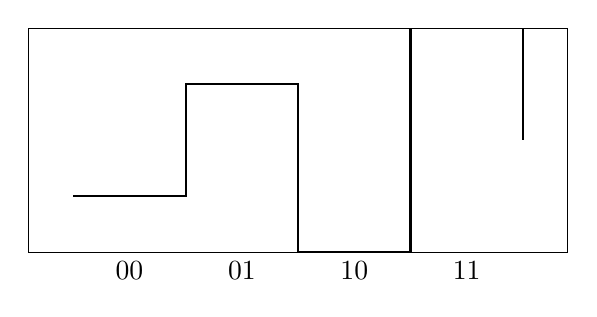
\begin{tikzpicture}
	\begin{axis}[xtick=\empty,ytick=\empty,yscale=.5,every extra x tick/.append style={major tick length=0pt},extra x ticks={.5,1.5,2.5,3.5},extra x tick labels={00,01,10,11},ymin=-2,ymax=2]
	\addplot [const plot,thick,draw=black]coordinates {(0,-1)(1,1)(2,-2)(3,2)(4,0)};
	\end{axis}
\end{tikzpicture}
\caption{Trasmissione multilivello quadripodale}
\end{figure}

La maggiore potenza disponibile consente in un sistema binario antipodale di distanziare le gaussiane in uscita dal filtro di ricezione tanto da diminuire di ordini di grandezza la probabilità di errore. Essendo la probabilità di errore legata alla varianza del rumore e alla distanza tra i livelli, avendo potenza in esubero è possibile inserire altri livelli a spaziatura tale da rispettare i limiti di probabilità d'errore e aumentare il numero di bit trasmessi da ciascun simbolo.\footnote{I livelli sono equispaziati in quanto la varianza del rumore non varia con la forma d'onda del simbolo trasmesso.} 

\begin{figure}[ht!]\centering
	\def\var{.707}
	\begin{tikzpicture}
	\pgfplotsset{set layers}
	\begin{axis}[scale=.5,xscale=4,xlabel=$V_C$,hide y axis,axis x line=middle,xtick={-3,-2,-1,1,2,3},ytick=\empty,xticklabels={$-3C$,$-2C$,$-C$,$C$,$2C$,$3C$},extra x ticks={-2,0,+2},extra x tick labels={},extra x tick style={grid=major},samples=300,xmin=-5.5,xmax=+5.5,domain=-5.5:+5.5]
	\addplot [name path=gauss00] {gauss(x,-3,\var)};
	\addplot [name path=gauss01] {gauss(x,-1,\var)};
	\addplot [name path=gauss10] {gauss(x,+1,\var)};
	\addplot [name path=gauss11] {gauss(x,+3,\var)};
	\path[name path=axis] (axis cs:-4,0)--node[above right,pos=0.5,pin=60:\footnotesize $P(01_R|00_T)$]{}node[above left,pos=0.25,pin=120:\footnotesize $P(10_R|00_T)$]{}(axis cs:4,0);
	\addplot[pattern=north west lines] fill between[of=gauss01 and axis,soft clip={domain=-4:-2}];
	\addplot[pattern=north east lines] fill between[of=gauss01 and axis,soft clip={domain=0:2}];
	\end{axis}
	\begin{axis}[scale=.5,xscale=4,xlabel=simboli,
	yshift=-0.4cm,axis x line=bottom,hide y axis,
	xtick={-3,-1,1,3},xticklabels={$10$,$00$,$01$,$11$},extra x ticks={-2,0,+2},extra x tick labels={soglia,soglia,soglia},extra x tick style={grid=major,yshift=-0.4cm},xmin=-5.5,xmax=+5.5]%
	\addplot coordinates {(0,0)};
	\end{axis}
	\end{tikzpicture}
	\caption{Modello statistico della decisione per un sistema a 4 livelli}
	\label{fig:trasmissione_numerica_modello_statistico_decisione_multilivello}
\end{figure}

Al ricevitore si dovrà discriminare con affidabilità sufficiente quale tra i quattro simboli è stato trasmesso in ogni periodo di simbolo. Definite le soglie tra le funzioni densità di probabilità associate alle possibili forme d'onda il sistema può decidere con una certa probabilità d'errore quale forma d'onda è stata inviata, in modo tale da individuare la configurazione di due cifre binarie associata al livello.

La probabilità d'errore è la probabilità di ottenere in uscita un livello diverso da quello trasmesso. Ciascun livello può essere confuso con qualunque livello precedente o successivo, ma risulta trascurabile la probabilità di confondere livelli tra loro non contigui. Si ha quindi che la probabilità d'errore è data dalla somma delle probabilità dell'evento confusione del livello $i$-esimo con la coppia dei livelli adiacenti per i livelli interni e con l'unico livello attiguo per i livelli esterni. Tale probabilità è pari all'area tagliata dalle soglie sulle code della gaussiana del livello $i$-esimo.

Si ha che la probabilità di errare livello in ricezione con $M$ livelli con simboli equiprobabili
\begin{equation}
p(\epsilon)=\sum_{i=1}^{M}p(\epsilon|S_i)p(S_i)=\frac{1}{M}\sum_{i=1}^{M}p(\epsilon|S_i)=\frac{(M-2)2p+2p}{M}=2p\frac{M-1}{M}
\end{equation}

Nell'ipotesi di associare a ciascuna forma d'onda una configurazione binaria secondo un codice Gray a distanza unitaria, in cui cambia un solo bit della configurazione tra simboli adiacenti, si ha che la probabilità di errare livello corrisponde con l'evento errare un bit del simbolo ricevuto. Avendo configurazioni di $n=\log_2{M}$ bit si ha che il \keyword[bit error rate]{bit error rate} o probabilità d'errore per un sistema ad $M=2^n$ livelli è
\begin{equation}
\text{BER}=\frac{p(\epsilon)}{\log_2{M}}=2p\frac{M-1}{M\log_2{M}}
\end{equation}

Confrontando le prestazioni di un sistema di trasmissione binario antipodale ($M=2$)  con i sistemi multilivello si ha che al costo di una maggiore potenza di trasmissione \footnote{si passa da una potenza di trasmissione $P_B$ ad una potenza di picco $P_M^p=(M-1)^2 P_B$ e una potenza media $P_M^m=\frac{M^2-1}{3}P_B$} si ottiene un minore \keyword{bit error rate} e una velocità di trasmissione $\log_2{M}$ superiore. La maggiore potenza di trasmissione rende i sistemi multilivello sensibili all'interferenza degli echi riflessi che possono avere potenza comparabile a quella dei livelli interni.
\begin{table}[ht]
\centering
\begin{tabular}{ccc}
$M$ & $p(\epsilon)$ & BER \\ \hline
2	& $p$ & $p$ \\
4	& $\frac{3}{2}p$ & $\frac{3}{4}p$ \\
8	& $\frac{7}{4}p$ & $\frac{7}{12}p$ \\
16	& $\frac{15}{8}p$ & $\frac{15}{32}p$ \\
\end{tabular}
\end{table}

\section{Scrambling}
Nell'ipotesi che i bit prodotti dalla sorgente dell'informazione non siano equiprobabili\footnote{ad esempio nella codifica ASCII il bit più significativo uguale a zero per la maggioranza dei caratteri d'uso comune} è possibile ottenerla applicando una operazione di \keyword[scrambling]{scrambling}: in fase di trasmissione si altera la sequenza di bit generata dalla sorgente scambiandone i bit con quelli di una sequenza pseudocasuale nota al mittente e al destinatario applicando l'operatore logico binario \keyword{XOR}, tale operazione reversibile è ripetuta in fase di ricezione per riottenere la sequenza originale.

\begin{table}[!ht]
	\centering
	\begin{tabular}{c}
		$a \oplus b = c$ \\ \hline
		$0 \oplus 0 = 0$ \\
		$0 \oplus 1 = 1$ \\
		$1 \oplus 0 = 1$ \\
		$1 \oplus 1 = 0$ 
	\end{tabular}
	\caption{Tabella di verità dell'operatore logico \keyword[operatore logico!XOR]{XOR}}
\end{table}

\clearpage
\section{Esercizio}
\begin{esercizio}
Un segnale analogico è campionato, quantizzato e codificato in un segnale binario \ac{PCM} con rappresentazione a $M=128$ livelli. Un impulso di sincronizzazione è è inviato dopo ogni campione.

Il segnale \ac{PCM} risultante è trasmesso su un canale in banda base $B=\SI{13}{\kilo\hertz}$ con modulazione di ampiezza multilivello \ac{PAM} quaternario con spettro a coseno rialzato.

Si vogliono determinare
\begin{enumerate}
	\item la velocità in bit/secondo di trasmissione dell'informazione (\keyword[bit rate]{bitrate}).
	\item la velocità di campionamento e la massima frequenza ammessa dal segnale analogico.
\end{enumerate}

Il segnale analogico ha campioni quantizzati a 7 bit a cui è aggiunto un bit di sincronizzazione tale da formare un parola di codice a 8 bit.

Il sistema trasmette simboli di 2 bit (\ac{PAM} quaternario) alla frequenza di cifra (\keyword{baud rate}) data dalla massima frequenza in banda base con forme d'onda di Nyquist dello spettro a coseno rialzato con $\delta=1$:
\[ B=\frac{1}{2 T_b}(1+\delta) \implies \text{baud rate}=\frac{1}{T_b}=\frac{2}{1+\delta}B=B=\SI{13}{\kilo\hertz}\]
\end{esercizio}
per cui la velocità di trasmissione del canale (\keyword{bitrate}): $\SI{26}{\kilo\bit\per\second}$

La velocità di campionamento o \keyword[sampling rate]{sampling rate} per parole di $\SI{8}{\bit}$:
\[f_\text{sampling}=\frac{\SI{26}{\kilo\bit\per\second}}{\SI{8}{\bit\per sample}}=\SI{3250}{\hertz}\]
Campionando almeno ad una frequenza doppia della massima frequenza del segnale analogico si ha \[f_s^\text{max}=\frac{f_S}{2}=\SI{1625}{\hertz}\]